\documentclass{article}

\usepackage[a4paper, top=1in, bottom=1in, left=0.7in, right=1.2in]{geometry}
\usepackage{forest}
\usepackage{amsmath}
\usepackage{graphicx}
\usepackage{tikz}
\usepackage[utf8]{inputenc}
\usepackage{tikz-qtree}
\usepackage{parskip}
\usepackage{arydshln}
\usepackage{float} % Add this package to control figure placement
\usetikzlibrary {arrows.meta,automata,positioning}
\title{Algoritmi v bioinformatiki - 1. Domača naloga}
\author{Jan Panjan}
\date{\today}

\begin{document}

\tikzset{
	node distance=2.6cm, % specifies the minimum distance between two nodes. Change if necessary.
	every state/.style={thick, fill=gray!10}, % sets the properties for each ’state’ node
	->, % makes the edges directed
	>={Stealth} % make arrow heads bold
}

\maketitle
\newpage

\begin{enumerate}
	\item \textit{Konstruirajte deterministični končni avtomat, ki v mRNK materialu prepozna
		zaključne kodone.}
		\begin{enumerate}
			\item \textbf{Grafično:}

			\begin{center}
				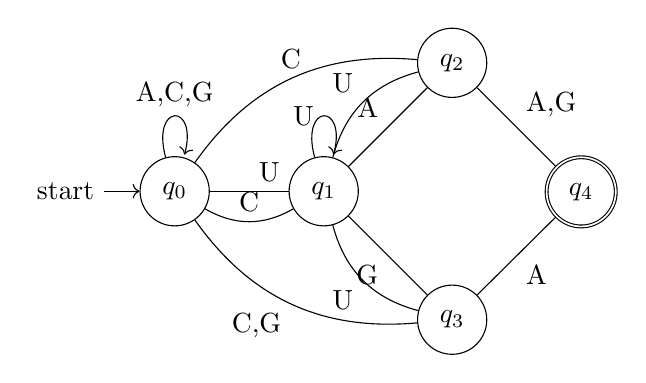
\begin{tikzpicture}
					\node[state, initial]   (q0)                     {$q_0$};
					\node[state] 			(q1) [right=of q0]       {$q_1$};
					\node[state] 	        (q2) [above right=of q1] {$q_2$};
					\node[state] 		    (q3) [below right=of q1] {$q_3$};
					\node[state, accepting] (q4) [below right=of q2] {$q_4$};

					\draw (q0) edge[loop above] node{A,C,G} (q0)
						(q0) edge[above right] node{U} (q1)

						(q1) edge[above, bend left] node{C} (q0)
						(q1) edge[above left] node{A} (q2)
						(q1) edge[below left] node{G} (q3)
						(q1) edge[loop above, left] node{U} (q1)

						(q2) edge[above left, bend right] node{U} (q1)
						(q2) edge[above right] node{A,G} (q4)
						(q2) edge[above, bend right] node{C} (q0)

						(q3) edge[below left, bend left] node{U} (q1)
						(q3) edge[bend left, below left] node{C,G} (q0)
						(q3) edge[below right] node{A} (q4);
				\end{tikzpicture}
			\end{center}

			\item \textbf{S formalnim opisom peterike $\left[ \Sigma, Q, q_0, F, \delta \right]$:}

				\begin{itemize}
					\item $\Sigma = \{ A, U, C, G \}$
					\item $Q = \{ q_1, q_2, q_3, q_4 \}$
					\item $q_0 = q_0$
					\item $F = \{ q_4 \}$
					\item stanja so pisana samo s številko in pot ki pripelje do
						končnega stanja je označena z rdečo barvo, da je bolj
						berljivo.

						\begin{tabular}{|c||c|c|c|c|}
							\hline
							$\delta$ & A & U & C & G \\
							\hline \hline
							0 & 0 & \textcolor{red}{1} & 0 & 0 \\
							\hline
							1 & \textcolor{red}{2} & 1 & 0 & \textcolor{red}{3} \\
							\hline
							2 & \textcolor{red}{4} & 1 & 0 & \textcolor{red}{4} \\
							\hline
							3 & \textcolor{red}{4} & 1 & 0 & 0 \\
							\hline
							4 & / & / & / & / \\
							\hline
						\end{tabular}
				\end{itemize}
		\end{enumerate}

	\newpage

	\item \textit{Kako se rešitev 1. naloge spremeni, če želimo s pomočjo končnega
			avtomata poiskati vse pojavitve zaključnih kodonov? Zapišite algoritem
			in ponazorite njegovo delovanje na delu mRNK AUAUAAUGCUUGA. Koliko
		zaključnih kodonov vsebuje dani mRNK?}

		Njegovo končno stanje se spremeni, tako da ponovno začne iskati vzorec, ko
		pride enkrat do
		končnega stanja. To je vidno grafično kot povezava od $q_4$ do $q_0$ in
		spremenjene vrednosti v zadnji vrstici $\delta-$tabele.

		\begin{enumerate}
			\item \textbf{Grafično:}

			\begin{center}
				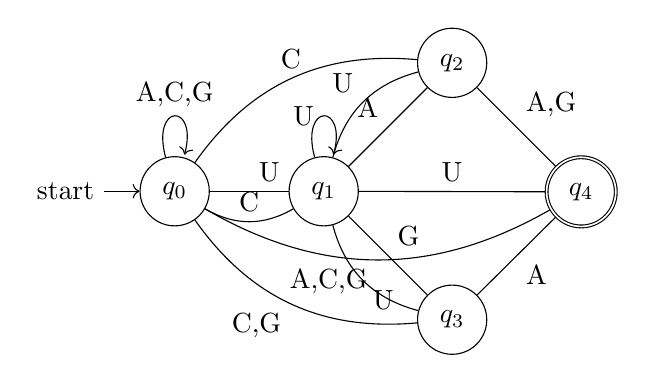
\begin{tikzpicture}
					\node[state, initial]   (q0)                     {$q_0$};
					\node[state] 			(q1) [right=of q0]       {$q_1$};
					\node[state] 	        (q2) [above right=of q1] {$q_2$};
					\node[state] 		    (q3) [below right=of q1] {$q_3$};
					\node[state, accepting] (q4) [below right=of q2] {$q_4$};

					\draw (q0) edge[loop above] node{A,C,G} (q0)
						(q0) edge[above right] node{U} (q1)

						(q1) edge[above, bend left] node{C} (q0)
						(q1) edge[above left] node{A} (q2)
						(q1) edge[above right] node{G} (q3)
						(q1) edge[loop above, left] node{U} (q1)

						(q2) edge[above left, bend right] node{U} (q1)
						(q2) edge[above right] node{A,G} (q4)
						(q2) edge[above, bend right] node{C} (q0)

						(q3) edge[below right, bend left] node{U} (q1)
						(q3) edge[bend left, below left] node{C,G} (q0)
						(q3) edge[below right] node{A} (q4)

						(q4) edge[above] node{U} (q1)
						(q4) edge[bend left, below left] node{A,C,G} (q0);
				\end{tikzpicture}
			\end{center}

			\item \textbf{S formalnim opisom peterike $\left[ \Sigma, Q, q_0, F, \delta \right]$:}

				\begin{itemize}
					\item $\Sigma = \{ A, U, C, G \}$
					\item $Q = \{ q_1, q_2, q_3, q_4 \}$
					\item $q_0 = q_0$
					\item $F = \{ q_4 \}$
					\item \begin{tabular}{|c||c|c|c|c|}
							\hline
							$\delta$ & A & U & C & G \\
							\hline \hline
							0 & 0 & \textcolor{red}{1} & 0 & 0 \\
							\hline
							1 & \textcolor{red}{2} & 1 & 0 & \textcolor{red}{3} \\
							\hline
							2 & \textcolor{red}{4} & 1 & 0 & \textcolor{red}{4} \\
							\hline
							3 & \textcolor{red}{4} & 1 & 0 & 0 \\
							\hline
							4 & 0 & 1 & 0 & 0 \\
							\hline
						\end{tabular}
				\end{itemize}
		\end{enumerate}

		\textbf{Algoritem za iskanje STOP kodonov v mRNA vzorcu:} algoritem deluje na osnovi
		$\delta-$tabele, tabela pa je lahko izgrajena neposredno iz grafičnega zapisa našege
		končenga avtomata oziroma preko formalnega zapisa peterke. Predpostavljam torej, da 
		je tabela za naš končni avtomat že izgrajena. Iskanje vzorca v besedilu AUAUAAUGCUUGA 
		poteka tako, da premaknemo končni avtomat v primerno stanje v tabeli glede na prebrani
		znak

		\begin{equation}
			\delta[q, c] = q'
		\end{equation}

		kjer je $q$ trenutno stanje, $c$ znak, ki ga preberemo iz besedila in $q'$ novo stanje.
		
		Dani vzorec mRNA vsebuje \textbf{dva} stop kodona: AUA\textcolor{red}{UAA}UGCU\textcolor{red}{UGA}

		\newpage

	\item \textit{Konstruirajte determinističen končni avtomat za naslednji
		nedeterminističen končni avtomat.}

		Deterministični končni avtomat iz nedeterminističnega izgradimo s pomočjo
		$\delta-$tabele tako da zapišemo vse neprazne podmnožice stanj. Za stanje
		npr. $1,2$ naredimo unijo sledečih stanj za $a$ in $b$, t.j $1,2,3$ in $2$., t.j $1,2,3$ in
		$2$. Da se izognemo pisanju nepotrebnih stanj, naredimo tabelo samo za dosegljiva
		stanja.

		\textbf{Nedeterminističen končni avtomat:}

		\begin{center}
			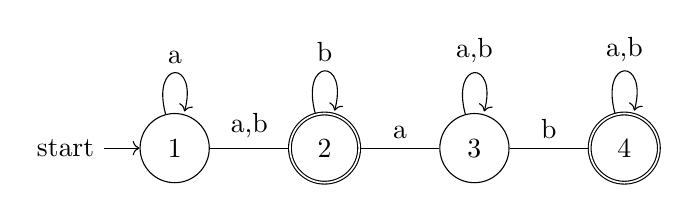
\begin{tikzpicture}
				\node[state, initial]   (q1)               {$1$};
				\node[state, accepting]	(q2) [right=of q1] {$2$};
				\node[state] 	        (q3) [right=of q2] {$3$};
				\node[state, accepting] (q4) [right=of q3] {$4$};

				\draw (q1) edge[loop above] node{a} (q1)
					(q1) edge[above] node{a,b} (q2)
					(q2) edge[loop above] node{b} (q2)
					(q2) edge[above] node{a} (q3)
					(q3) edge[loop above] node{a,b} (q3)
					(q3) edge[above] node{b} (q4)
					(q4) edge[loop above] node{a,b} (q4);
			\end{tikzpicture}

			\textbf{$\delta-$tabela:}

			\begin{tabular}{|c||c|c|}
				\hline
				$\delta$ & a & b \\
				\hline\hline
				1 & 1,2 & 2 \\
				\hline
				2 & 3 & 2 \\
				\hline
				3 & 3 & 3,4 \\
				\hline
				4 & 4 & 4 \\
				\hline
				1,2 & 1,2,3 & 2 \\
				\hline
				3,4 & 3,4 & 3,4 \\
				\hline
				1,2,3 & 1,2,3 & 2,3,4 \\
				\hline
				2,3,4 & 3,4 & 2,3,4 \\
				\hline
			\end{tabular}
		\end{center}

		Končna stanja sta $2$ in $4$, zato bo imel novi končni avtomat za končna
		stanja vsa stanja, ki vsebujejo tako $2$ ali $4$.

		Zgodi se, da stanje $4$ odpade, saj nobeno stanje ne vodi vanj.

		\textbf{Determinističen končni avtomat:}

		\begin{center}
			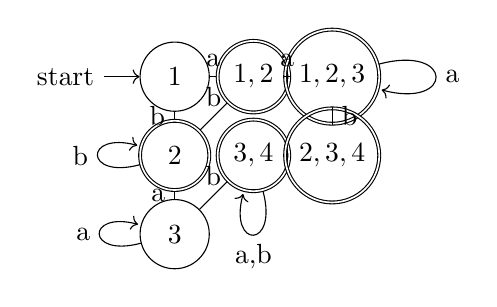
\begin{tikzpicture}
				\node[state, initial] (1) {$1$};
				\node[state, accepting] (2) [below of=1] {$2$};
				\node[state] (3) [below of=2] {$3$};
				\node[state, accepting] (12) [right of=1] {$1,2$};
				\node[state, accepting] (123) [right of=12] {$1,2,3$};
				\node[state, accepting] (34) [below of=12] {$3,4$};
				\node[state, accepting] (234) [below of=123] {$2,3,4$};

				\draw (1) edge[left] node{b} (2)
					(1) edge[above] node{a} (12)
					(12) edge[above] node{b} (2)
					(12) edge[above] node{a} (123)
					(123) edge[loop right] node{a} (123)
					(123) edge[right] node{b} (234)
					(2) edge[loop left] node{b} (2)
					(2) edge[left] node{a} (3)
					(3) edge[loop left] node{a} (3)
					(3) edge[above] node{b} (34)
					(34) edge[loop below] node{a,b} (34);
			\end{tikzpicture}
		\end{center}

		\newpage

	\item \textit{Poleg postopka z uporabo končnih avtomatov, poznamo tudi druge načine, kako
			odgovoriti na vprašanje "Kje in kolikokrat se vzorec p pojavi v besedilu t"? Naj bo naše
		besedilo $t$ = ACCACCGACGCCCGA.}

		\begin{enumerate}
			\item \textit{Za vzorec $p$ = CCGA, ponazorite delovanje algoritma KMP tako, da poiščete
					vzorec $p$ v besedilu $t$ in opišite, kako nam pri tem pomaga funkcija $\pi$.
				Kolikokrat in kje se vzorec $p$ pojavi v besedilu $t$?}

				\textbf{KMP} ali \textbf{Knuth-Moriss-Prath-ov algoritem} deluje na principu najdaljše predpone vzorca,
				ki je tudi pripona v dotedaj preiskanem besedilu. Z uporabo $\pi-$funkcije se
				algoritem izogne nepotrebnim primerjavam znakov v besedilu, za katere že vemo, da
				se ujemajo na začetku vzorca.

				Psevdokoda za algoritem KMP izgleda tako:

				\begin{verbatim}
					def KMP(t, p):
						n = |t|
						m = |p|
						pi = Construct(p) // izgradi zgornji pi-seznam
						r = []            // seznam ki hrani začetne indekse
											 //         kjer se pojavi ujemanje
						q = 0

						for i = 1 to n - 1:
							while q > 0 and p[q + 1] is not t[i]:
									q = pi

							   if p[q + 1] == t[i]:
									q += 1

								  if q == m:
									   r = r.add(i - q + 1)

						   return r
				\end{verbatim}

				S funkcijo $\pi$ najdemo najdaljšo predpono vzorca, ki je tudi njegova najdaljša
				pripona. Za naš vzorec izgleda tako:

				\begin{center}
					\begin{tabular}{c|c c c c}
						$p$ & C & C & G & A \\
						\hline
						$\pi(p)$ & 0 & 1 & 0 & 0 \\
					\end{tabular}
				\end{center}

				\newpage

				Potek algoritma je opisan z naslednjo tabelo:

				\begin{center}
					\begin{tabular}{|c|c|c|c|c|l|}
						\hline
						$q$ & $i$ & $p[q+1]$ & $t[i]$ & match & action \\
						\hline\hline
						0 & 1 & C & A & No & incr i \\
						\hline
						0 & 2 & C & C & Yes & incr q,i \\
						\hline
						1 & 3 & C & C & Yes & incr q,i \\
						\hline
						2 & 4 & G & A & No & $q=\pi[2]=1$ \\
						\hline
						1 & 4 & C & A & No & $q=\pi[1]=0$ \\
						\hline
						0 & 4 & C & A & No & incr i \\
						\hline
						0 & 5 & C & C & Yes & incr q,i \\
						\hline
						1 & 6 & C & C & Yes & incr q,i \\
						\hline
						2 & 7 & G & G & Yes & incr q,i \\
						\hline
						3 & 8 & A & A & Yes & incr q,i \\
						\hline
						4 & 9 & $\epsilon$ & C & No & $r.add(i-q+1)$, $q=\pi[4]$ \\
						\hline
						0 & 9 & C & C & Yes & incr q,i \\
						\hline
						1 & 10 & C & G & No & $q=\pi[1]$ \\
						\hline
						0 & 10 & C & G & No & incr i \\
						\hline
						0 & 11 & C & C & Yes & incr q,i \\
						\hline
						1 & 12 & C & C & Yes & incr q,i \\
						\hline
						2 & 13 & G & C & No & $q=\pi[2]$ \\
						\hline
						1 & 13 & C & C & Yes & incr q,i \\
						\hline
						2 & 14 & G & G & Yes & incr q,i \\
						\hline
						3 & 15 & A & A & Yes & incr q,i \\
						\hline
						4 & 16 & $\epsilon$ & $\epsilon$ & - & $r.add(i-q+1)$, $i=m:STOP$ \\
						\hline
					\end{tabular}
				\end{center}

				Vzorec se pojavi dvakrat v našem besedilu. Algoritem najde ujemanja na indeksih
				\textbf{5} in \textbf{12}.

				\newpage

			\item \textit{Zgradite priponsko drevo za besedilo $t$. Opišite, kako s pomočjo
					priponskega drevesa učinkovito odgovorimo na vprašanje "Kje in kolikokrat se v
				besedilu $t$ pojavi aminokislina prolin?"}

				\textbf{Priponsko drevo} izgradimo tako, da najprej najdemo vse pripone našega besedila $t$,
				nato pa jih (po abecednem vrstnem redu) dodajamo v drevo z začetkom v korenu.
				Pripone, ki imajo enako pripono bodo sledile istemu poddrevesu, a ga bodo nato
				razcepile na več podvej. V listih drevesa hranimo začetni indeks pripone.

				Vse pripone našega besedila:

				\begin{center}
					\begin{tabular}[t]{c|l}
						1. & ACCACCGACGCCCGA\$ \\
						2. & CCACCGACGCCCGA\$ \\
						3. & CACCGACGCCCGA\$ \\
						4. & ACCGACGCCCGA\$ \\
						5. & CCGACGCCCGA\$ \\
						6. & CGACGCCCGA\$ \\
						7. & GACGCCCGA\$ \\
						8. & ACGCCCGA\$ \\
						9. & CGCCCGA\$ \\
						10. & GCCCGA\$ \\
						11. & CCCGA\$ \\
						12. & CCGA\$ \\
						13. & CGA\$ \\
						14. & GA\$ \\
						15. & A\$ \\
						16. & \$ \\
					\end{tabular}
				\end{center}

				Indeksi urejeni po abedecnem vrstnem redu:

				\begin{center}
					16, 15, 1, 4, 8, 3, 2, 11, 12, 5, 13, 6, 9, 14, 7, 10
				\end{center}

				Iz tega zdaj izgradimo priponsko drevo. Zgostil sem ga, da je bolj
				pregleden:

				\begin{figure}[H] % Use [H] to force the figure to stay in place
					\centering
					\includegraphics[width=1\textwidth]{suffix-tree.jpg}
				\end{figure}

				\newpage

			\textbf{Kje in kolikokrat se v besedilu pojavi aminokislina prolin:}
				prolin kodira več kodonov in sicer CCU, CCC, CCA ter CCG. Da najdemo vse
				njegove pojavitve v besedilu se spustimo po izgrajenem drevesu. Začnemo v 
				korenu ter se pomikamo v pravo poddrevo glede na prebrani znak. Ko smo v
				notranjem vozlišču, kjer se vzorec konča, se spustimo do vseh listov v 
				trenutnem poddrevesu, tako da najdemo vse začetne indekse kjer se pojavi 
				vzorec v besedilu.

				\begin{enumerate}
					\item CCU se v besedilu \textbf{ne pojavi}
					\item CCC ima začetek na \textbf{11.} indeksu
					\item CCA na \textbf{2.} indeksu
					\item CCG na \textbf{5.} in \textbf{12.} indeksu
				\end{enumerate}

				\newpage

			\item \textit{Zgradite priponsko polje za besedilo $t$. Opišite, kako s pomočjo
					priponskega polja učinkovito odgovorimo na vprašanje "Kje in kolikokrat se v
				besedilu $t$ pojavi aminokislina prolin?"}

				\textbf{Priponsko polje} izgradimo iz indeksov, ki smo jih dali v liste priponskega drevesa,
				tako da pripone uredimo po abecednem vrstnem redu.

				\begin{center}
					\begin{tabular}{|c||c|c|c|c|c|c|c|c|c|c|c|c|c|c|c|c|c|}
						\hline
						indeks v polju (m) & 0 & 1 & 2 & 3 & 4 & 5 & 6 & 7 & 8 & 9 & 10 & 11 & 12 & 13 & 14 & 15 \\
						\hline
						indeks v besedilu (i) & 16 & 15 & 1 & 4 & 8 & 3 & 2 & 11 & 12 & 5 & 13 & 6 & 9 & 14 & 7 & 10 \\
						\hline
					\end{tabular}
				\end{center}

				\textbf{Kje in kolikokrat se v besedilu pojavi aminokislina prolin:} ujemanja najdemo
				z bisekcijo. Vsako iteracijo izberemo srednji indeks v polju (oziroma levi, če je
				velikost polja soda) in primerjamo njegovo pripono z vzorcem. Če je vzorec manjši glede
				na abecedni vrstni red, se pomaknemo v levo polovico polja in odstranimo srednji indeks
				ter desno polovico (obratno, če je vzorec večji). Če pride do ujemanja z vzorcem, se
				pomaknemo v levo polovico polja in nadaljujemo z bisekcijo. Iskanje se konča, ko zmanjka
				indeksov v polju.

				\textbf{CCU:}

				\begin{center}
					\begin{tabular}{|c|c||c|c|c|}
						\hline
						m & i & primerjava & ujemanje & akcija \\
						\hline
						\hline
						7 & 11 & $CCC\dots < CCU$ & ne & desno \\
						\hline
						11 & 6 & $CGA\dots > CCU$ & ne & levo \\
						\hline
						9 & 5 & $CCA\dots < CCU$ & ne & desno \\
						\hline
						10 & 13 & $CGA\dots > CCU$ & ne & levo = end \\
						\hline
					\end{tabular}

					Ni ujemanj.
				\end{center}

				\textbf{CCC:}

				\begin{center}
					\begin{tabular}{|c|c||c|c|c|}
						\hline
						m & i & primerjava & ujemanje & akcija \\
						\hline
						\hline
						7 & 11 & $CCC\dots = CCC$ & ja & levo \\
						\hline
						3 & 4 & $ACC\dots < CCC$ & ne & desno \\
						\hline
						5 & 3 & $CAC\dots < CCC$ & ne & desno \\
						\hline
						6 & 2 & $CCA\dots < CCC$ & ne & desno = end \\
						\hline
					\end{tabular}

					Ujemanje najdemo na 11. indeksu.
				\end{center}

				\textbf{CCA:}
				
				\begin{center}
					\begin{tabular}{|c|c||c|c|c|}
						\hline
						m & i & primerjava & ujemanje & akcija \\
						\hline
						\hline
						7 & 11 & $CCC\dots > CCA$ & ne & levo \\
						\hline
						3 & 4 & $ACC\dots < CCA$ & ne & desno \\
						\hline
						5 & 3 & $CAC\dots < CCA$ & ne & desno \\
						\hline
						6 & 2 & $CCA\dots = CCA$ & ja & desno = end \\
						\hline
					\end{tabular}

					Ujemanje najdemo na 2. indeksu.
				\end{center}

				\textbf{CCG:}

				\begin{center}
					\begin{tabular}{|c|c||c|c|c|}
						\hline
						m & i & primerjava & ujemanje & akcija \\
						\hline
						\hline
						7 & 11 & $CCC\dots < CCG$ & ne & desno \\
						\hline
						11 & 6 & $CGA\dots > CCG$ & ne & levo \\
						\hline
						9 & 5 & $CCG\dots = CCG$ & ja & levo \\
						\hline
						8 & 12 & $CCG\dots = CCG$ & ja & levo = end \\
						\hline
					\end{tabular}

					Ujemanji najdemo na 5. in 12. indeksu.
				\end{center}

				\newpage

			\item \textit{Besedilo t želimo zakodirati. Kateri način kodiranja nam bo dal 
			najkrajši zapis:}

			• \textit{uporaba fiksne dolžine kod,} \\
			• \textit{uporaba Huffmanovega algoritma,} \\
			• \textit{uporaba Burrows-Wheeler transformacije, algoritma MTF in 
			Huffmanovega algoritma (v tem vrstnem redu).}

			\textit{Odgovor ustrezno utemeljite.}

			\textbf{Fiksna dolžina kod:} naša abeceda ima 4 znake (A, C, G, U) oziroma 5,
			če dodamo še \$, ki ga potrebujemo za označevanje konca besedila. Vsak znak
			zakodiramo z enakim številom bitov. V tem primeru bi bila 2-bita premalo ($2^2=4$),
			zato potrebujemo vsaj 3-bite ($2^3=8$).

			\begin{center}
				\begin{tabular}{c|c}
					znak & koda \\
					\hline
					A & 000 \\
					C & 001 \\
					G & 010 \\
					U & 011 \\
					\$ & 100 \\
				\end{tabular}
			\end{center}

			Vsak znak iz abecede je predstavljen z 8-biti (1-bajt). Dolžina našega besedila
			je 16 znakov, kar pomeni, da potrebujemo 16 bajtov oziroma 128 bitov za normalen
			zapis besedila. Če ga s pomočjo kodiranja z 3-biti zakodiramo, dobimo
			$16 \cdot 3 = $ \textbf{48-bitov}, kar je 80 bitov prihranka!

			\textbf{Huffmanov algoritem:} Huffmanov algoritem deluje na principu frekvenc 
			znakov. Je tako imenovano entropijsko kodiranje. S pomočjo frekvenc znakom
			dodelimo dolžine kod, ki so obratno sorazmerne z njihovimi frekvencami (višja
			frekvenca implicira krajšo kodo).

			\begin{center}
				\begin{tabular}{c|c}
					znak & frekvenca ($t_i$) \\
					\hline
					A & 4 \\
					C & 8 \\
					G & 3 \\
					U & 0 \\
					\$ & 1 \\
				\end{tabular}
			\end{center}

			Iz frekvenc izgradimo drevo, tako da združujemo znake z najnižjimi frekvencami
			v eno vozlišče. Na koncu dobimo drevo, ki ga uporabimo za kodiranje znakov
			(v vozliščih je zapisana vsota frekvenc znakov). 

			\begin{center}
				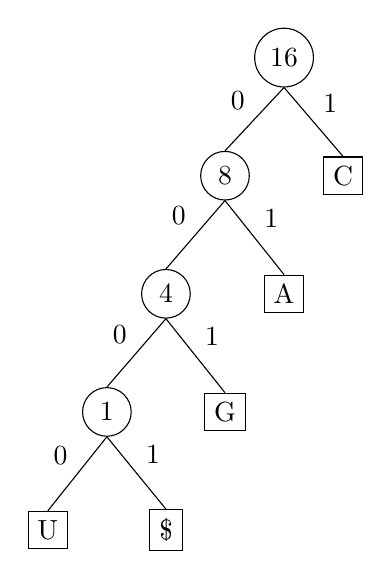
\begin{tikzpicture}
					\node[circle, draw] {16}
						child {node[circle, draw] {8}
							child {node[circle, draw] {4}
								child {node[circle, draw] {1}
									child {node[rectangle, draw] {U} edge from parent node[above left] {0}}
									child {node[rectangle, draw] {\$} edge from parent node[above right] {1}}
									edge from parent node[above left] {0} % Left edge labeled 0
								}
								child {node[rectangle, draw] {G} edge from parent node[above right] {1}}
								edge from parent node[above left] {0} % Left edge labeled 0
							}
							child {node[rectangle, draw] {A} edge from parent node[above right] {1}}
							edge from parent node[above left] {0} % Left edge labeled 0
						}
						child {node[rectangle, draw] {C} edge from parent node[above right] {1}}; % Right edge labeled 1
				\end{tikzpicture}
			\end{center}
			
			Kode dobimo tako, da se iz korena sprehodimo do listov, kjer se nahaja pripadajoči 
			znak.  Na poti do lista dodamo 0, če gremo levo in 1, če gremo desno. 

			\begin{center}
				\begin{tabular}{c|c|l}
					znak & frekvenca ($t_i$) & koda \\
					\hline
					A & 4 & 01 \\
					C & 8 & 1 \\
					G & 3 & 001 \\
					U & 0 & 0000 \\
					\$ & 1 & 0001 \\
				\end{tabular}
			\end{center}

			Iz teh kod zdaj sestavimo zakodirano besedilo:

			\begin{center}
				HE(t) = 01110111001011001111001010001
			\end{center}

			Dolžino besedila najhitreje izračunamo preko frekenc znakov in dolžin kod:

			\begin{align*}
				& t_A \cdot |01| + t_C \cdot |1| + t_G \cdot |001| + t_U \cdot |0000| + t_{\$} \cdot |0001| \\
				=& \ 4 \cdot 2 + 8 \cdot 1 + 3 \cdot 3 + 0 \cdot 4 + 1 \cdot 4 \\
				=& \ 8 + 8 + 9 + 0 + 4 \\
				=& \ 29
			\end{align*}

			Zakodirano besedilo ima torej \text{29-bitov}, kar je boljše kot 48-bitov pri fiksni
			dolžini kod.

			\textbf{Burrows-Wheeler transformacija:} Burrows-Wheeler transformacija je algoritem,
			ki uporabimo za predprocesiranje besedila, da je nadaljne kodiranje bolj
			učinkovito. Deluje na principu t.i. \textit{rotacij besedila}. Najprej izgradimo vse 
			rotacije besedila, nato pa jih uredimo po abecednem vrstnem redu. Na koncu
			odčitamo zadnje znake vseh rotacij, da dobimo transformirano besedilo.

			\begin{center}
				\begin{tabular}{|c|l||c|l|l|}
					\hline
					i & rotacije & i & urejeno & zadnji znak \\
					\hline
					1. & ACCACCGACGCCCGA\$ & 16. & \$\dots & A  \\
					\hline
					2. & CCACCGACGCCCGA\$A & 15. & A\$\dots & G  \\
					\hline
					3. & CACCACGCCCGA\$AC & 1. & ACCA\dots & \$ \\
					\hline
					4. & ACCGACGCCCGAA\$ACC & 4. & ACCG\dots & C  \\
					\hline
					5. & CCGACGCCCGAA\$ACCA & 8. & ACG\dots & G  \\
					\hline
					6. & CGACGCCCGAA\$ACCAC & 3. & CA\dots & C  \\
					\hline
					7. & GACGCCCGA\$ACCACC & 2. & CCA\dots & A  \\
					\hline
					8. & ACGCCCGA\$ACCACCG & 11. & CCCG\dots & G  \\
					\hline
					9. & CGCCCGA\$ACCACCGA & 12. & CCGA\$\dots & C  \\
					\hline
					10. &  GCCCGA\$ACCACCGAC & 5. & CCGAC\dots & A  \\
					\hline
					11. &  CCCGA\$ACCACCGACG & 13. & CGA\$\dots & C  \\
					\hline
					12. &  CCGA\$ACCACCGACGC & 6. & CGAC\dots & C \\
					\hline
					13. &  CGA\$ACCACCGACGCC & 9. & CGC\dots & A  \\
					\hline
					14. &  GA\$ACCACCGACGCCC & 14. & GA\$\dots & C  \\
					\hline
					15. &  A\$ACCACCGACGCCCG & 7. & GAC\dots & C  \\
					\hline
					16. &  \$ACCACCGACGCCCGA & 10. & GC\dots & C  \\
					\hline
				\end{tabular}
			\end{center}

			\begin{center}
				$BWT(t)=AG\$CGCAGCACCACCC$
			\end{center}

			To zdaj zakodiramo s pomočjo \textbf{MTF (move-to-front) algoritma}. MTF algoritem deluje tako, da
			se sprehodimo čez transformirano besedilo, istočasno pa urejamo in dodajamo znake v pravem vrstnem
			redu v pomožno tabelo. Prebran znak premaknemo na vrh tabele in odčitamo indeks iz katerega smo 
			ga premaknili. Ostale znake premaknemo eno mesto navzdol (prva vrstica v tabeli predstavlja naše 
			transformirano besedilo).

			\begin{center}
				\begin{tabular}{c c||cccccccccccccccc}
					1 & \$ & A & G & \$ & C & G & C & A & G & C & A & C & C & A & C & C & C \\
					2 & A & \$ & A & G & \$ & C & G & C & A & G & C & A & A & C & A & A & A \\
					3 & C & C & \$ & A & G & \$ & \$ & G & C & A & G & G & G & G & G & G & G \\
					4 & G & G & C & C & A & A & A & \$ & \$ & \$ & \$ & \$ & \$ & \$ & \$ & \$ & \$ \\
					5 & U & U & U & U & U & U & U & U & U & U & U & U & U & U & U & U & U \\
					\hline
					  &   & 2 & 4 & 3 & 4 & 3 & 2 & 4 & 3 & 3 & 3 & 2 & 1 & 2 & 2 & 1 & 1 \\
				\end{tabular}
			\end{center}
			
			Zadnja vrstica je rezultat MTF algoritma: $MTF(BWT(t))=2434324333212211$.

			To zaporedje števil nato zakodiramo s pomočjo Huffmanovega algoritma, tako kot prej:

			\begin{center}
				\begin{tabular}{c|c}
					znak & frekvenca ($t_i$) \\
					\hline
					1 & 3 \\
					2 & 5 \\
					3 & 5 \\
					4 & 4 \\
				\end{tabular}
			\end{center}

			Iz frekvenc ustvarimo drevo:

			\begin{center}
				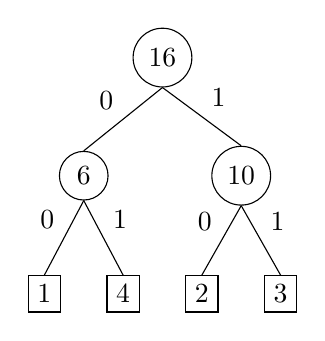
\begin{tikzpicture}[level/.style={sibling distance=20mm/#1}]
					\node[circle, draw] {16}
						child {node[circle, draw] {6}
							child {node[rectangle, draw] {1}
									edge from parent node[above left] {0} 
							}
							child {node[rectangle, draw] {4}
									edge from parent node[above right] {1}
							}
							edge from parent node[above left] {0}
						}
						child {node[circle, draw] {10} 
							child {node[rectangle, draw] {2}
								edge from parent node[above left] {0} 
							}
							child {node[rectangle, draw] {3}
								edge from parent node[above right] {1}
							}
							edge from parent node[above right] {1}
						};
				\end{tikzpicture}
			\end{center}

			Dobimo pripadajoče kode:

			\begin{center}
				\begin{tabular}{c|c|c}
					znak & frekvenca ($t_i$) & koda \\
					\hline
					1 & 3 & 00 \\
					2 & 5 & 10 \\
					3 & 5 & 11 \\
					4 & 4 & 01 \\
				\end{tabular}
			\end{center}

			Zakodirano besedilo je torej:
			\begin{center}
				HE(MTF(BWT(t))) = 10011101111001111111100010100000
			\end{center}

			Dolžino zakodiranega besedila ponovno izračunamo iz frekvenc in dolžin kod:

			\begin{align*}
				& t_1 \cdot |00| + t_2 \cdot |10| + t_3 \cdot |11| + t_4 \cdot |01| \\
				=& \ (3 + 5 + 5 + 3) \cdot 2 \\
				=& \ 16 \cdot 2 \\
				=& \ 32
			\end{align*}

			Besedilo transformirano z Burrows-Wheeler transformacijo in zakodirano z MTF ter
			Huffmanovim algoritmom je dolgo  \textbf{32-bitov}, kar je slabše od 29-bitov pri samem
			Huffmanovem algoritmu.

			\begin{quote}
				Mislim, da je razlog za slabši rezultat Burrows-Wheeler transformacije ta,
				da je naše besedilo prekratko. Burrows-Wheeler transformacija je bolj učinkovita 
				pri daljših besedilih, ki vsebujejo veliko ponavljajočih se znakov, saj jih lahko tako 
				uredi skupaj (na primer AA\$GGGGCCCCC...). Ker BWT ne privede do boljše ureditve, MTF 
				kodiranje ni efektivno (ta v svoj prid izkorišča dolga ponavljajoča-se zaporedja, podobno
				kot RLE - run-length encoding.).
			\end{quote}

			\textbf{Zaključek:} Najboljše kodiranje dobimo s pomočjo Huffmanovega algoritma, ki nam da 
			zakodirano besedilo dolžine 29-bitov.

		\end{enumerate}

\end{enumerate}
\end{document}
